\documentclass[conference]{IEEEtran}
\usepackage{graphicx}
\graphicspath{ {images/} }

\title{MAP-4384 Quiz 1}
\author{Tyler Lukasiewicz }

\begin{document}

\maketitle

    \begin{abstract}
        This is an abstract and the words shuold be bold. And if I write just a little bit more, it will make autoatically.
    \end{abstract}
    \section{Approximation of the Derivative}
    \label{sec:Approximation of the Derivative}

        The derivative of a continuous function $f$ is defined by the following equation. 

        \begin{equation}
            f'(x) = \lim _ {h \to 0 } \frac{f(x+h) - f(x)}{h} 
        \end{equation}

        So, if we would like to approximate the derivative of a continuous function $f$ at a point $x$, then we may use the formula

        \begin{equation}
            f'(x) \approx  f_a(x) = \frac{f(x+h) - f(x)}{h} 
        \end{equation}

        For some $h$. As $h \to 0$, $f_a'(x) \to f(x)$. We can determine the error of our approximation,  $\epsilon$ with the formula 

        \begin{equation}
            \epsilon = |f'(x) - f_a(x)|
        \end{equation}

        Below is a graph of the error, $\epsilon$ of the  aprixmate derivative of $\sin (\pi / 3)$.

        \begin{figure}[!ht]
           \begin{center}
               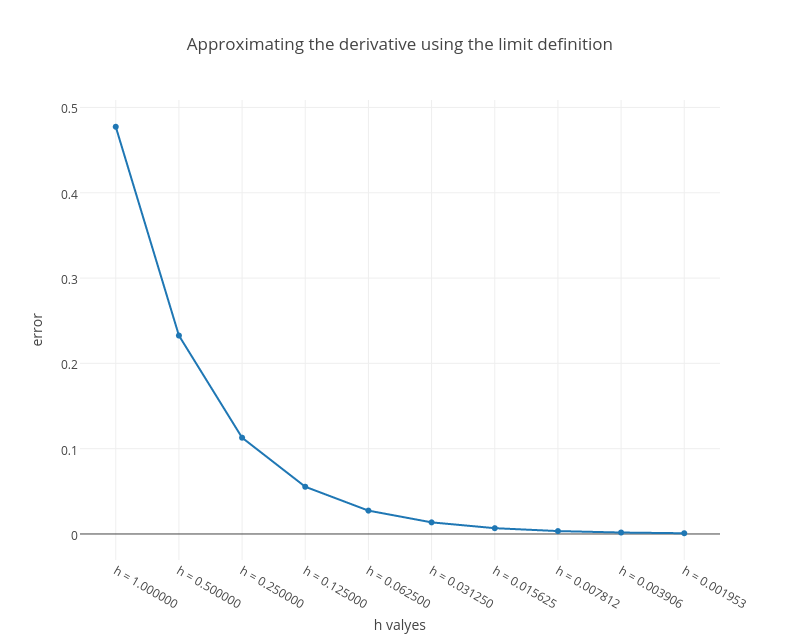
\includegraphics[scale=.50]{graph}
           \end{center}
            \label{fig:1}
        \end{figure}

        As we can see, as $h \to 0$, $\epsilon \to 0$.

\end{document}
